\icode{E-MD-CA-L2-261114-002}
楼梯口一倾斜的天花板与水平地面成 $\theta =$ \,\qty{37}{\degree}，一装潢工人手持木杆绑着刷子粉刷天花板，工人所持木杆对刷子的作用力始终保持竖直向上，大小为 $F = $ \,\qty{10}{N}，刷子的质量为 $m = $\,\qty{0.5}{kg}，刷子可视为质点，刷子与板间的动摩擦因数 $\mu$ 为 $0.5$，天花板长为 $L = $\,\qty{4}{m}，取 $\sin$\,\qty{37}{\degree}=0.6，$\cos$\,\qty{37}{\degree}=0.8，试求：
\begin{enumerate}
	\item 刷子沿天花板向上的加速度；
	\item 刷完天花板的时间。
\end{enumerate}

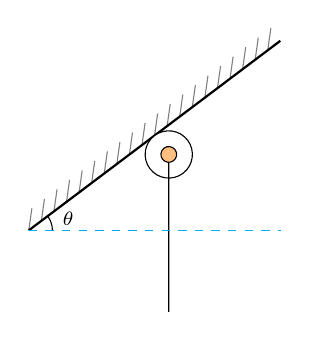
\begin{tikzpicture}[>=stealth,font=\scriptsize]
	\begin{scope}[rotate=37]
		\foreach \x in {0,.2,...,3.8}
			\draw[gray] (\x,0)--++(.2,.2);
		\draw[thick] (0,0)--(4,0);
		\draw[fill=white] (2,-.3)coordinate(o) circle(.3);
		\draw (o)--++(-127:2);
		\draw[fill=orange!50] (o) circle(.1);
	\end{scope}
	\draw[dashed,cyan] (0,0)--(3.2,0);
	\draw (.3,0) arc(0:37:.3);
	\node at(.5,.15){\(\theta\)};
\end{tikzpicture}
\begin{answer}
    （1）（2）
\end{answer}